\documentclass[main.tex]{subfiles}
\begin{document}
Rappel : filtre analogique linéaire

\[ e(t) \rightarrow \boxed{G(p)} \rightarrow s(t) \]
\[ s(t) = g(t)*e(t) \]
\[ S(p) = G(p) E(p) \]

\section{Premières propriétés}

\begin{thm}
Si on applique un échantillonnage en entrée de e(t),
\[s(t) = g(t) * e^*(t) \]
\begin{enumerate}
\item $s^*(t) = g^*(t) * e^*(t)$ où $g^*(t)$ est l’échantillonnage de $g(t)$

\item $s_n = g_n * e_n = \sum_ {k=0}^n g_{n-k}e_k$

\end{enumerate}
\end{thm}

\begin{proof}
\begin{enumerate}
\item
\[g^*(t) * e^*(t) = \int_0^{\infty} g^*(t-\tau)e^*(\tau)d\tau = ... \]

\item
\begin{align*}
s^*(t) & = s(t)\sum_{k=0}^{\infty}\delta_0(t-kT_e) = \sum_{k=0}^{\infty}s_k\delta_0(t-kT_e)
\intertext{Or, $ s(t) = \int_0^{\infty}g(t-\tau)e^*(\tau)d\tau $ avec $ e^*(t) = \sum_ {k=0}^{\infty}e_k\delta_0(t-kT_e)$}
\text{donc } s(t) & = \int_ 0^{\infty}g(t-\tau)(\sum_{k=0}^{\infty}e_k\delta_0(\tau-kT_e))d\tau \\
& = \sum_ {k=0}^{\infty}e_k \int_0^{\infty} g(t-\tau) \delta_0(\tau-kT_e) d\tau \\
& = \sum_ {k=0}^{\infty}e_k g(t-kT_e) \\
s_n = s(nT_e) & = \sum_ {k=0}^{\infty}e_kg((n-k)T_e) = \sum_ {k=0}^{\infty}e_kg_{n-k}
\end{align*}

\end{enumerate}
\end{proof}

Application : Discrétisation d'un système analogique avec CNA + BOZ

\begin{figure}[h!]
\centering
\begin{tikzpicture}
\sbEntree{E}


\sbBloc{cna}{CNA, BOZ}{E}
\sbRelier[$u_k$]{E}{cna}

\sbBloc[3]{sys}{G(p)}{cna}
\sbRelier[$u(t)$]{cna}{sys}

\sbBloc[3]{can}{CAN}{sys}
\sbRelier[$y(t)$]{sys}{can}

\sbSortie[3]{S}{can}
\sbRelier[$y_k$]{can}{S}


\end{tikzpicture}
\caption{Discrétisation d'un système analogique}
\end{figure}

Hypothèse : Synchronisation des convertisseurs

\[ u_k \rightarrow \boxed{H(z)} \rightarrow y_k \]

\subsection*{Fonction de transfert pour asservissement numérique}

On cherche à déterminer la fonction de transfert $H(z)=\frac{Y(z)}{U^*(z)}$ de l'asservissement numérique suivant :


\begin{figure}[h!]
\centering
\begin{tikzpicture}
\sbEntree{E}

\sbBloc{calc}{CNA}{E}
\sbRelier[$u_k$]{E}{calc}

\sbBloc[3]{boz}{$B_0(p)$}{calc}
\sbRelier[$u^*(t)$]{calc}{boz}

\sbBloc[3]{sys}{$G(p)$}{sys}
\sbRelier{boz}{sys}

\sbBloc[3]{can}{CAN}{sys}
\sbRelier[$y(p)$]{sys}{can}

\sbSortie[3]{S}{can}
\sbRelier[$y^*(t)$]{can}{S}


\end{tikzpicture}
\caption{Asservissement numérique}
\end{figure}

\begin{thm}
\[ \boxed{H(z) = (1-z^{-1}) Z[^*L^{-1}[\frac{G(p)}{p}]]} \]
\end{thm}

\begin{preuve}
\begin{align*}
Y(p) & = B_0(p)G(p)U^*(p) \\
& = (1 - e^{-T_ep})\frac{G(p)}{p}U^*(p) \\
& = \frac{G(p)}{p}U^*(p)-\frac{G(p)}{p}U^*(p)e^{-T_ep}
\intertext{On pose $ \tilde{G}(p) = \frac{G(p)}{p} $ }
Y(p) & = \tilde{G}(p)U^*(p) - \tilde{G}(p)U^*(p)e^{-T_ep}
\end{align*}

Avec $\tilde{Y}(p) = \tilde{G}(p)U^*(p)$, par transformation inverse de Laplace,
\begin{align*}
\tilde{y}(t) & = \tilde{g}(t)*u^*(t) \\
\tilde{y}_n & = \tilde{g}_n*u_n \\
\tilde{Y}(z) & = \tilde{G}(z)U(z)\\
\text{Ainsi, } Y(z) & = \tilde{Y}(z) - z^{-1}\tilde{Y}(z) \\
& = (1-z^{-1})\tilde{Y}(z) \\
H(z) & = (1-z^{-1})\tilde{G}(z) \\
H(z) & = (1-z^{-1})Z[^*L^{-1}[\tilde{G}(p)]]
\end{align*}
\end{preuve}

\medskip
\noindent Remarque : comment choisir $T_e$ ? Tout système physique peut être représenté par un filtre passe-bas :
\[ \boxed{ \text{Règle empirique : } 6f_c \leq f_e \leq 24f_c } \]

\subsection*{Propriétés des systèmes discrétisés}

\begin{enumerate}
\item Un système analogique linéaire reste linéaire après discrétisation.
\item L'ordre du système est conservé.
\item Les pôles du système discrétisé $p_d$ sont liés aux pôles du système analogique $p_c = e^{T_e p_c}$ (cela vient de $z=e^{T_ep}$). Attention, c'est faux pour les zéros  !
\item La discrétisation d'une association en série n'est pas identique à la mise en série des discrétisés.
\end{enumerate}

\section{Obtention d'une fonction de transfert en z à partir d'une équation récurrente}

\[a_ny_{k+n} + ... + a_1y_{k+1}+a_0y_k = b_mu_{k+m} + ... + b_1u_{k+1} + b_0u_k \]
\[ \text{ avec } a_i,b_j \in \mathbb{R}, a_n \neq 0 \]

Par causalité, on a $n \geq m$. \\

Rappel : Théorème d'avance
\[ Z[u_{k+d|d\in\mathbb{N}^*}] = z^d U(z) - z^d \sum_{i=0}^{d-1}u_iz^{-i} \]

On applique la transformée en $z$ à ($EQ_n$) = $a_ny_{k+n} + ... + a_1y_{k+1}+a_0y_k$
\[
\begin{array}{lcll}
a_n y_{k+n} & & a_nz^nY(z) & - a_n [y_0...y_{n-1}][z^n...z]^T \\
+ a_{n-1} y_{k+N-1} & & + a_{n-1}z^{n-1}Y(z) & - a_{n-1} [0, y_0...y_{n-2}][z^n...z]^T  \\
... & \quad \rightarrow \quad TZ \quad \rightarrow \quad & ... & ... \\
+ a_1 y_{k+1} & & + a_1z^{n-1}Y(z) & - a_1 [0, ...,0,y_0][z^n...z]^T  \\
+ a_0 y_k & & +a_0zY(z) \\
\hline
TZ(EQ_n) & = & (\sum_{l=0}^na_lz^l)Y(z) & - CI_y(z)
\end{array}
\]

On fait de même avec ($EQ_m$) = $b_mu_{k+m} + ... + b_1u_{k+1} + b_0u_k$.

Conditions initiales données : les $y_k, k = 0,...,n-1$ et $u_k,k=0,...,m-1$

\begin{align*}
CIy(z) & = \sum_{j=0}^{n-1} ( \sum_{l=0}^j a_{n-l}y_{l-j}) z^{n-j}  \\
CIu(z) & = \sum_{j=0}^{m-1} ( \sum_{l=0}^j b_{m-l}u_{l-j}) z^{n-j}
\end{align*}

Ainsi, en posant \[A(z) = \sum_{l=0}^n a_lz^l \text{ et } B(z) = \sum_{l=0}^m b_lz^l \]

\begin{align*}
& A(z)Y(z) - CIy(z) = B(z)U(z) - CIu(z) \\
& \boxed{Y(z) = \frac{B(z)}{A(z)} U(z) + \frac{CIy(z)-CIu(z)}{A(z)}}
\end{align*}

On pose $G(z)=\frac{B(z)}{A(z)}$, appelée fonction de transfert du système.

\begin{align*}
Y(z) &  = G(z)U(z) + \frac{CI(z)}{A(z)} \\
& \text{ où } CI(z) = CIy(z) - CIu(z) \\
& \text{ À CI nulles, } Y(z) = G(z) U(z)
\end{align*}

\subsection*{Définitions}
Les pôles (zéros) du système sont les racines de $A(z)$  ($B(z)$).

Le gain statique (si défini) est \( \lim_{z\rightarrow 0}G(z)\).

Lorsqu'il n'y a plus de simplifications possibles entre pôles et zéros dans G(z), on parle de fonction de transfert minimale. Alors, le degré de A(z) désigne l'ordre du système.

\section{Réponse temporelle de système à temps discret}

On considère le système à temps discret :
\[u_k \rightarrow \boxed{G(z)} \rightarrow y_k \]

\[G(z) = \frac{B(z)}{A(z)} \text{ et } A(z) = \sum_{l=0}^n a_lz^l, B(z) = \sum_{l=0}^m b_lz^l\]

\subsection{Calcul à partir de la relation de récurrence}

On effectue un changement de variable muet pour exprimer $y_k$ en fonction des instants précédents.
\[a_ny_{k+n} + ... + a_1y_{k+1}+a_0y_k  = b_mu_{k+m} + ... + b_1u_{k+1} + b_0u_k \]
\[a_ny_k = -a_{n-1}y_{k-1}-...-a_1y_{k-n+1}-a_0y_{k-n} + b_mu_{k+m-n} + ... + b_1u_{k-n+1} + b_0u_{k-n}\]
Intérêt : pratique pour le calcul en temps réel (simulation, implantation systèmes embarqués...). Les CI $y_{-1}, y_{-2}...$ sont à préciser

\subsection{Calcul à partir de la fonction de transfert}
Si les CI sont nulles :
\begin{align*}
Y(z) & = G(z)U(z) \\
y_k & = Z^{-1}[G(z)U(z)]
\end{align*}
En pratique, on effectue une décomposition en éléments simples de $\frac{Y(z)}{z}$ et on applique $Z^{-1}[.]$ à $Y(z)$ en utilisant le tableau des transformées en z usuelles.\\

Exemple :
\begin{align*}
\intertext{On cherche la réponse impulsionnelle ($u_k=\delta_k$) de }
G(z)& = \frac{1}{(z-1)(z-2)}
\intertext{On effectue la décomposition en éléments simples de $\frac{Y(z)}{z}$}
\frac{Y(z)}{z} & = \frac{1}{z(z-1)(z-2)} \\
& = \frac{1}{2z} - \frac{1}{2(z-1)} + \frac{1}{2(z-2)} \\
Y(z) & = \frac{1}{2} - \frac{1}{2}\frac{z}{z-1} + \frac{1}{2} \frac{z}{z-2} \\
y_k &= \frac{1}{2}\delta_k + \frac{1}{2}2^k -1
\end{align*}

SI les CI non nulles et connues :
\begin{align*}
Y(z) & = G(z) U(z) + \frac{CIy(z)-CIu(z)}{A(z)} \\
y_k &= Z^{-1}[G(z) U(z) + \frac{CIy(z)-CIu(z)}{A(z)}]
\end{align*}

\subsection{Par décomposition modale}

\begin{align*}
G(z) & = \frac{b_mz^m + ... + b_0}{a_nz^n + ... + a_0} = \frac{B(z)}{A(z)} \\
& = \frac{K(z-z_1)^{\alpha_1}(z-z_2)^{\alpha_2}...(z-z_r)^{\alpha_r}}{(z-p_1)^{\gamma_1}(z-p_2)^{\gamma_2}...(z-p_q)^{\gamma_q}} \text{ avec } \sum_1^q \gamma_i = n, \sum_1^r \alpha_i = m
\end{align*}

$\gamma_i$ est la multiplicité algébrique du pôle $p_i \in \mathbb{C}$.

$\alpha_i$ est la multiplicité algébrique du zéro $z_i \in \mathbb{C}$

Avec l'hypothèse $a_n=1$, $A(z)$ est un polynôme appelé Monique.

\begin{align*}
\frac{Y(z)}{z} & = \frac{G(z)U(z)}{z} \text{ où U(z) quelconque, de pôles } r_1,...,r_u \\
\text{ d'où } Y(z) & = Y(0) + \sum_{i=1}^q G_i(z) + \sum_{i=1}^{r_u}U_i(z)
\end{align*}

Remarque : $U(z)$ influence la décomposition de $G(z)$ et vice-verse.

\begin{align*}
G_i(z) & = \sum_{j=1}^{\gamma_i}\frac{c_{ij}z}{(z-p_j)^j} \\
g_{i_k} & = Z^{-1}[G_i(z)] \\
& = (c_0 + c_1k + ... + c_{\gamma_i - 1}k^{\gamma_i - 1})p_i^k
& = P_i(k)p_i^k
\end{align*}

$g_{i_k}$ correspond à l'évolution de la sortie $y_k$ due au pôle $p_i$ : mode $p_i$.

\medskip

La sortie $y_k$ est construite à partir de la contribution de chaque mode (et du type d'entrée)
\[ y_k = Y(0)\delta_k + \sum_{i=1}^q g_{i_k} + Z^{-1}[\sum_{i=1}^{r_u}U_i(z)] \]
où

$\sum_{i=1}^q g_{i_k}$ est l'excitation des modes par l'entrée $y_k$

$Z^{-1}[\sum_{i=1}^{r_u}U_i(z)]$ le régime forcé par $u_k$

\subsubsection{Mode réel}

\begin{itemize}
\item $|p_i|<1 \Rightarrow P_i(k)p_i^k \rightarrow_{\infty} 0$ : mode convergent
\item $|p_i|>1 \Rightarrow P_i(k)p_i^k $ divergence exponentielle
\item $ |p_i| = 1 et P_i(k) = c_0$ constant $\rightarrow$ mode entretenu (ni convergence, ni divergence)
\item $ |p_i| = 1 $ et $ \gamma_i > 1, P_i(k)p ^k \rightarrow $ divergence polynomiale
\begin{itemize}
\item Si $p_i > 0$ alors $ P_i(k)p_i^k$ tend à être du même signe : mode apériodique
\item Si $p_i < 0$ alors $P_i(k)p_i^k = (-1)^k |p_i|^k P_i(k)$ change de signe en fonction de la parité de k : mode oscillant
\item Si $p_i = 0 \rightarrow P_i(k)p_i^k = 0 \forall
k\geq 1$ : mode à réponse pile
\end{itemize}
\end{itemize}
Remarque : un pôle discret nul $p_i = 0$ possède un équivalent en temps continu à partie réelle infiniment négative :
\[p_i = e^{T_ep_{ci}} = 0 \Leftrightarrow p_{i} \rightarrow - \infty\]

\subsubsection{Mode complexe}
À un pôle $p_i$ complexe correspond son conjugué $\overline{p_i}$ :
\[P_{a_i}(k)p_i^k + P_{b_i}(k)\overline{p_i}^k = ... = P(k)\rho_i^k\sin(k\theta_i+\phi\]
où $p_i = \rho_ie^{j\theta_i}$ et $\phi$ dépend du contexte.
\begin{itemize}
\item $|p_i| = \rho_i > 1$ : divergence
\item $|p_i| = \rho_i < 1$ : convergence en $\rho_i^k$
\item $|p_i| = \rho_i = 1$
\begin{itemize}
\item si multiplicité de $p_i = 1$ : mode entretenu
\item si multiplicité de $p_i > 1$ : divergence
\end{itemize}
\item $\theta_i \neq 0$ oscillation à la fréquence $\theta$
\end{itemize}

\section{Stabilité}

\begin{defin}[Stabilité EBSB]
Un système discret est stable au sens EBSB si pour toute entrée $u_k$ bornée, $y_k$ reste bornée.
\end{defin}

\begin{thm}[Stabilité et réponse impulsionnelle]
Un système est stable au sens EBSB si et seulement si sa réponse impulsionnelle est absolument sommable, c'est-à-dire $\sum_ {k=0}^{\infty}|g_k|<\infty$
\end{thm}


\subsection*{Théorème : stabilité et pôles}
\begin{thm}[Stabilité et pôles]
Un système discret est stable au sens EBSB si et seulement si tous les pôles de sa fonction de transfert en $z$ sont à l'intérieur du cercle unité (strictement, pas sur le cercle).
\end{thm}

Remarque : cela suppose le calcul des pôles de $G(z) = \frac{B(z)}{A(z)}$

\begin{figure}[h!]
\centering
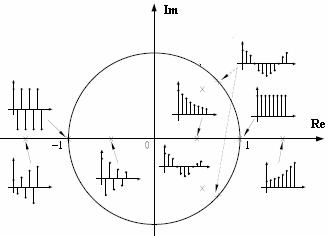
\includegraphics[scale=0.8]{polesenz.jpg}
\caption{Allure de la réponse temporelle en fonction de la position des pôles dans le plan $z$}
\end{figure}

\subsection*{Critère de Jury}
\emph{À savoir utiliser, voir polycopié.}

\subsection*{Critère de Routh-Hurwitz}
\emph{À connaître par coeur, voir polycopié.}\\

Rappel : En temps continu, le critère de Routh-Hurwitz permet de déterminer le nombre de racines instables de l'équation caractéristique, c'est-à-dire à partie réelle strictement positive.\\

Transformation en w :
\begin{align*}
z & = \frac{1+w}{1-w} ,\quad w \neq 1 \\
w & = \frac{z-1}{z+1} ,\quad z \neq -1
\end{align*}

Cette transformation transforme le disque unité du plan en $z$, en le preuvei-plan ouvert gauche du plan en $w$.

Cette transformation étant bijective, on l'utilise pour appliquer le critère de Routh au polynôme en la variable $w$.

\subsection*{Critère de stabilité de Schur-Cohn}
\emph{Non exigible, voir polycopié.}

\subsection*{Critère de stabilité de Nyquist}
\emph{À connaître par coeur, voir polycopié.}
\section{Transposition des méthodes analogiques}

\subsection{Approximation du BOZ par un retard équivalent}

On rappelle l'expression de la fonction de transfert du BOZ :
\begin{align*}
B_0(p) & = \frac{1-e^{-T_ep}}{p} \\
& = \frac{e^{-\frac{T_e}{2}p} ( e^{\frac{T_e}{2}p} - e^{-\frac{T_e}{2}p})}{p} \\
\text{ Or, } & e^{-\frac{T_e}{2}p} = 1 - \frac{T_e}{2}p + o(\frac{T_e}{2}p) \\
& e^{-\frac{T_e}{2}p} = 1 + \frac{T_e}{2}p + o(\frac{T_e}{2}p) \\
\text{Donc } & \boxed{ B_0(p)  \approx T_e e^{-\frac{T_e}{2}p}}
\end{align*}

\subsection{Approximation de Padé pour les retards}

Cette approximation repose sur le développement de Taylor du terme de retard exponentiel. Elle fournit une fraction rationnelle causale.

À l'ordre 1,
\[ e^{-T_ep} = \frac{e^{-\frac{T_e}{2}p}}{e^{+\frac{T_e}{2}p}} = \frac{1 - \frac{T_e}{2}p}{1 + \frac{T_e}{2}p} \]

À l'ordre 2,
\[ e^{-T_ep} = \frac{1 - \frac{T_e}{2}p + \frac{T_e^2}{8}p^2}{1 + \frac{T_e}{2}p + \frac{T_e^2}{8}p^2}  \]

Application au BOZ :
\[\boxed{B_0(p) \approx \frac{T_e}{1+\frac{T_e}{2}p}}\]

Conséquence : on peut donc appliquer les résultats des systèmes analogiques sur le système équivalent obtenu.

\subsection{Correction numérique obtenue par discrétisation approchée d'un correcteur continu}

\subsubsection*{Approximation de l'opérateur intégral}

\begin{align*}
x(t) & = \int_ 0^t e(\tau)d\tau\\
x_k & = x(kT_e) = \int_ 0^{kT_e} e(\tau)d\tau \\
x_k & = \sum_{j=0}^k e_jT_e
\end{align*}


\subsubsection*{Approximation d'Euler arrière}
\begin{align*}
\frac{de(t)}{dt} & = \frac{e_k - e_{k-1}}{T_e} \\
pE(p) & = \frac{1-z^{-1}}{t_e}E(z)
\end{align*}
\[ \boxed{p = \frac{z-1}{zT_e}} \]

\subsubsection*{Approximation d'Euler avant}
\begin{align*}
\frac{de(t)}{dt}& = \frac{e_{k+1}-e_k}{T_e} \\
pE(p) & = \frac{z-1}{T_e}E(z)
\end{align*}
\[ \boxed{p = \frac{z-1}{T_e} } \]


\subsubsection*{Approximation de Tustin}
\begin{align*}
x_k - x_{k-1} & = \frac{1}{2}(e_k + e_{k-1})T_e \\
(1-z^{-1})X(z) & = \frac{T_e}{2}(1+z^{-1})E(z) \\
X(z) & = \frac{T_e}{2}\frac{1+z^{-1}}{1-z^{-1}}E(z) \\
& = \frac{T_e}{2}\frac{z+1}{z-1}E(z)
\end{align*}

D'où \[ \boxed{p = \frac{2}{T_e}\frac{z-1}{z+1}} \]

Remarque : semblable à la transformation en $w$.

Remarque : les approximations de $p$ induisent des distorsions fréquentielles.

Exemple : correcteur continu $R_C(p)$ \\
$R_d(z) = R_c(p) |_{p=\frac{2}{T_e} \frac{z-1}{z+1}}$

Réponse fréquentielle : $ z=e^{T_ep}, p=j\omega$

\begin{align*}
R_d(e^{jT_e\omega}) & = R_c(\frac{2}{T_e} \frac{jT_e\omega-1}{jT_e\omega+1}
\\
\frac{jT_e\omega-1}{jT_e\omega+1} & = j\tan(\frac{T_e}{2}\omega) \\
R_d(e^{jT_e\omega}) & = R_c(j\frac{2}{T_e} \tan(\frac{T_e}{2})\omega)
\\
& = R_c(j\tilde{\omega}) \text{ où } \tilde{\omega} = \frac{2}{T_e}\tan(\frac{T_e}{2}\omega)
\end{align*}

$\tilde{\omega}$ est une "pseudo-pulsation" qui varie de 0 à $+\infty$ lorsque $\omega$ varie de 0 à $\frac{\pi}{2}$. Cela correspond à une distorsion de l'échelle fréquentielle.

Approximation de Tustin adaptée à la pulsation $\omega_c$

On voudrait que $R_d(e^{j\omega_cT_e}) = R_c(j\omega_c)$, alors
\[p \leftarrow \frac{\omega_c}{\tan(\frac{\omega_cT_e}{2})}\frac{z-1}{z+1}\]
\[R_c(j\frac{\omega_c}{\tan(\frac{\omega_cT_e}{2}})) = R_c(j\omega_c)\]

Approximation par correspondance pôle-zéro

Exemple :
\begin{align*}
R_c(p) & = \frac{p+a}{p+b} \\
z & = e^{T_ep} \\
R_d(z) & = \frac{z-e^{-T_ea}}{z-e^{-T_eb}} \alpha \\
\text{Gain statique : } & \lim_{z\rightarrow1}R_d(z) = \alpha \frac{1-e^{-T_ea}}{1-e^{-T_eb}} = \lim_ {p\rightarrow 0} R_c(p) = \frac{a}{b} \\
\alpha & = \frac{a}{b} \frac{1-e^{-T_ea}}{1-e^{-T_eb}}
\end{align*}

En résumé, on construit $R_d(z)$ avec la même structure que $R_c(p)$ en temres de zéros, pôles et gain statique.
Précaution à prendre lorsque le degré du numérateur de $R_c(p)$ est inférieur au degré du dénominateur de $R_c(p)$ (i.e. $R_c(p)$ strictement propre)

Exemple :
\begin{align*}
R_c(p) & = \frac{p+a}{(p+b)(p+c)} \\
R_d(p) & = \frac{(z+1)(z - e^{-T_ea})}{(z-e^{-T_eb)(z-e^{-T_ec})}}\alpha \\
R_d(1) = R_c(0) \rightarrow \alpha = ...
\end{align*}
Le terme $(z+1)$ est ajouté pour permettre d'avoir le même gain de $R_d(z)|_{z=e^{jT_e\frac{\pi}{T_e}}} = R_c(j\omega)|_{\omega \rightarrow \infty}$ (correspondance du gain haute fréquence).

En conclusion, le choix d'une approximation dépend beaucoup des caractéristiques (zéros, ordre,...) du système.
\end{document}
